\documentclass{article}

\usepackage{amsmath} % Math stuff
\usepackage{amssymb} % math symbols
\usepackage{graphicx} % include graphics
\graphicspath{{./}{./includes}} % default directory

\usepackage{hyperref} % include links

\usepackage{geometry} % change layout
\geometry{margin=2.5cm} % same as defaul word document

\usepackage{lipsum} % for dummy text
\usepackage{enumitem} % chage lists % noitemsep / nosep
\setlist{itemsep=0.2em} % between lines

\title{My knowledge}
\author{Fabrizio Cortesi}

% All the common commands are situated here
%
% for an arrow in text mode
\newcommand\arrow{$\,\Rightarrow\,$ }
%
% overbracing in text mode
\newcommand\textover[2]{$\overbrace{\text{#1}}^{\text{#2}}$}
%
% vectro creation 
\newcommand\vecTwo[2]{\begin{pmatrix} #1 \\ #2 \end{pmatrix}}
\newcommand\vecThree[3]{\begin{pmatrix} #1 \\ #2 \\ #3 \end{pmatrix}}
%
% absolute value
\newcommand\abs[1]{\lvert #1 \rvert}

\begin{document}

\maketitle

\section*{Introduction}

Hello there!

\tableofcontents

\section{Mathematics}

\subsection{Basic}
\subsubsection{Nomenclature}


\begin{gather*}
\begin{alignedat}{1}
    %addition
    \overbrace{
        \overbrace{
        \text{augend}+\text{addend}
        }^{\text{summands}}=\text{sum}
    }^{\text{addition}} \qquad
    %
    &
    % subtraction
    \overbrace{
        \overbrace{
        \text{minuend}-\text{subtrahend}
        }^{\text{terms}}=\text{difference}
    }^\text{subtraction}
    \\\\
    %
    % multiplication 
    \overbrace{
        \overbrace{
        \text{multiplier}\cdot\text{multiplicand}
        }^{\text{factors}}=\text{difference}
    }^\text{multiplication} \qquad
    %
    &
    % division
    \overbrace{
        \overbrace{
        \dfrac{\text{nominator}}{\text{denominator}}
        }^\text{fraction}=\dfrac{\text{dividend}}{\text{divisor}}=\text{ratio, quotient}
    }^\text{division}
\end{alignedat} \\\\
%
% expt
\overbrace{
    \text{base}^\text{exponent} = \text{power}
}^\text{exponentiation} \qquad
% sqrt
\overbrace{
    \sqrt[\text{\scriptsize degree}]{\text{radicand}}=\text{root}
}^{n\text{th root}} \qquad
% log
\overbrace{
    \log_\text{base}(\text{numerus})=\text{logarithm}
}^\text{logarithm}
\\\\
%
% absolute value
\overbrace{
    |x| = \begin{cases} x, & \text{if } x \geq 0 \\ -x, & \text{if } x < 0 \end{cases}
}^\text{absolute value} \qquad
%
% facotrial
\overbrace{
    n! = \prod_{i=1}^{n} i
}^\text{factorial} \qquad
%
% modulos
\overbrace{
    a \equiv b \pmod{n}
}^\text{modulos}
\\\\
%
% Summation
\overbrace{
    \sum_{i=m}^n a_i = a_m + a_{m+1} + \cdots + a_{n-1} + a_n
}^\text{summation} \qquad
%
% multiplication
\overbrace{
    \prod_{i=m}^n a_i = a_m \cdot a_{m+1} \cdot \cdots \cdot a_{n-1} \cdot a_n
}^\text{product of a sequence}
\\\\
%
% Derivative
\overbrace{
    f'(x) = \lim_{h \to 0} \frac{f(x+h) - f(x)}{h}
}^\text{derivative} \qquad
%
% Integral
\overbrace{
    \int_a^b f(x) dx
}^\text{integral}
\end{gather*}

\subsubsection{Greek letters}

\begin{center}
\begin{tabular}{ccccccccc}
    \multicolumn{9}{c}{Greek Letters} \\
    Name & Alpha & Beta & Gamma & Delta & Epsilon & Zeta & Eta & Theta \\
    Lowercase & $\alpha$ & $\beta$ & $\gamma$ & $\delta$ & $\epsilon$ & $\zeta$ & $\eta$ & $\theta$ \\
    Uppercase & $A$ & $B$ & $\Gamma$ & $\Delta$ & $E$ & $Z$ & $H$ & $\Theta$ \\
    \\
    Name & Iota & Kappa & Lambda & Mu & Nu & Xi & Omicron & Pi \\
    Lowercase & $\iota$ & $\kappa$ & $\lambda$ & $\mu$ & $\nu$ & $\xi$ & $o$ & $\pi$ \\
    Uppercase & $I$ & $K$ & $\Lambda$ & $M$ & $N$ & $\Xi$ & $O$ & $\Pi$ \\
    \\
    Name & Rho & Sigma & Tau & Upsilon & Phi & Chi & Psi & Omega \\
    Lowercase & $\rho$ & $\sigma$ & $\tau$ & $\upsilon$ & $\phi$ & $\chi$ & $\psi$ & $\omega$ \\
    Uppercase & $P$ & $\Sigma$ & $T$ & $\Upsilon$ & $\Phi$ & $X$ & $\Psi$ & $\Omega$ \\
\end{tabular}
\end{center}



\subsubsection{Number sets}

\begin{equation*}
\newcommand\eq{&\,=\kern 2pt&}
%
\begin{alignedat}{3}
    &\mathbb{N}^+ \eq \left\{1, 2, 3,4,\dots\right\} \eq \text{Natural numbers} \\
    &\mathbb{N}_0 \eq \left\{0, 1, 2,\dots\right\} \eq \text{Whole numbers } \\
    &\mathbb{Z} \eq \left\{-1, 2, -3,\dots\right\} \eq \text{Integer numbers} \\
    &\mathbb{Q} \eq \left\{-\tfrac{4}{7}, 3,\dots\right\} \eq \text{Rational numbers} \\
    &\mathbb{R} \eq \left\{\pi, \sqrt{2},\dots\right\} \eq \text{Real numbers} \\
    &\mathbb{C} \eq \left\{a + bi \right\} \eq \text{Complex numbers}
\end{alignedat}
\end{equation*}


\subsubsection{Powers, roots and logs}

\begin{gather*}
    a^{-n} = \dfrac{1}{a^n} \qquad
    a^{\frac{ b}{ c}} = \left( \sqrt[ c]{a} \space\right)^b =  \sqrt[ c]{a^b}
    \\\\
    a^n \cdot a^m = a^{m+n} \qquad
    \sqrt[n]{a}\cdot\sqrt[m]{a} = \sqrt[\uproot{15}\frac{1}{\frac{1}{n}+\frac{1}{m}}]{a} \qquad
    \log_n(a\cdot b)=\log_n(a) + \log_n(b)
    \\\\
    a^n : a^m = a^{m-n} \qquad
    \sqrt[n]{a}:\sqrt[m]{a} = \sqrt[\uproot{15}\frac{1}{\frac{1}{n}-\frac{1}{m}}]{a} \qquad    
    \log_n(a : b)=\log_n(a) - \log_n(b) 
    \\\\
    a^n \cdot b^n = \left( a \cdot b\right)^n \qquad
    \sqrt[n]{a} \cdot \sqrt[n]{b} = \sqrt[n]{a \cdot b} \qquad
    \log_n(a)\cdot\log_m(a) = \log_?(?)
    \\\\
    a^n : b^n = \left(a : b\right)^n \qquad
    \sqrt[n]{a} : \sqrt[n]{b} = \sqrt[n]{a : b} \qquad
    \log_n(a):\log_m(a) = \log_n(m)
    \\\\ 
    \left( a^n \right) ^ m = a^{m\space\cdot\space n}\qquad
    \sqrt[n]{\sqrt[m]{a}} = \sqrt[n \cdot m]{a}  \qquad
    \log_{a^n}(b^m) = \frac{m\cdot\log_a(b)}{n}
    \\\\
    x^{\log_b(y)}=b^{\log_b(x)\log_b(y)}=y^{\log_b(x)}
    \\\\
    \log_m(x) = \dfrac{\log_n(x)}{\log_n(m)}
\end{gather*}


\subsubsection{Trigonometry}

\begin{gather*}
    \sin(x) = \dfrac{O}{H} \qquad \cos(x) = \dfrac{A}{H} \qquad \text{tan}(x) = \dfrac{O}{A} \\ \space \\
    \\
    \dfrac{\text{sin}(\alpha)}{a} = \dfrac{\text{sin}(\beta)}{b}\kern 1em \text{if given angel isn't opposite to longer side} \implies \textbf{2 solutions} \\ \space \\
    \\
    c = \sqrt{a^2+b^2-2ab\cdot\text{cos}(\gamma)}
\end{gather*}

\subsection{Equations}

Indeterminate \& coefficients
$\frac{1}{x}, 2^n$ are not polynomials

Grundmenge: $\mathbb{G}$ \\
Function domain, Defintionsmenge: $\mathbb{D}$ \\
Solution set, Lösungsmege: $\mathbb{L}$ \\
\\
From the function domain we remove where the denominator is 0 or the radicand negative is
\\
Taking a root loses solutions $x^2 = 4$ because $x = 2$ loses $x = -2$ \\
For the same reason exponentiation adds solutions

Inequality invert > to < if multiplied/divided by negative numbers

For roots and absolute divide equation in positive and negative side

where $>$ becomes $<$ and for x $<$ $=>$ and, x $>$ $=>$ or

x = x 
0 = 1

\subsection{Polynomials}

\subsubsection{Lineaer}

Definition: $y = f(x) = 
\overbrace{mx+q}^\text{standard} =
\overbrace{m(x-u) + v}^\text{point}$

From $P_1(x_1,y_1)$ and $P_2(x_2, y_2)$ one can get $m = \dfrac{\Delta y}{\Delta x} = \dfrac{y_2-y_1}{x_2-x_1}$
From $m$ and $P(x, y)$ one can get $q = y-mx$
X-intersect: $x = q$
Y-intersect: $y = -\dfrac{q}{m}$
Preserve vector addition: $f(a + b) = f(a) + f(b)$
Preserve scalar multiplication: $a\cdot f(b) = f(a\cdot b)$
90° slope: $m_2 = -\dfrac{1}{m}$

\subsubsection{Quadratic}

Definition: $y = f(x) = 
\overbrace{ax^2+bx+c}^\text{standard}=
\overbrace{a(x-x_1)(x-x_2)}^\text{factored}=
\overbrace{a(x-u)^2+v}^\text{vertex}$

$x = \dfrac{-b\pm\sqrt{b^2-4ac}}{2a}$

Discriminant: $D = b^2-4ac$

%X-intersect: $\begin{rcases}
%  &x_1 = \dfrac{-b+\sqrt{D}}{2a}, x_2 = \dfrac{-b-\sqrt{D}}{2a} &\text{if } D > 0 \\
%  &x = \dfrac{-b}{2a}                                           &\text{if } D = 0 \\
%  &\varnothing                                                  &\text{if } D < 0
%\end{rcases}$
Y-intersect: $y = c$
Vertex: $S, V = P\left(-\dfrac{b}{2a}, f(x)\right) = P\left(-\dfrac{b}{2a}, -\dfrac{b^2-4ac}{4a}\right)$

- if $a > 0$, parabola opens upwards
- if $a < 0$, parabola opens downwards

\subsection{Vectors}

\begin{gather*}
\vec{v} = \vec{0v} = \vecTwo{x}{y} \\\\
\vec{AB} = \vecTwo{B_x - A_x}{B_y - A_y} \qquad \vec{BA} = \vecTwo{A_x - B_x}{A_y - B_y}\\\\
\vec{v_1} + \vec{v_2} = \vec{v_3} = \begin{pmatrix} v_{1x} + v_{2x} \\ v_{1y} + v_{2y} \end{pmatrix} \\\\
n\cdot\vec{v}=\vecTwo{n\cdot v_x}{n\cdot v_y} \\\\
\abs{a}
\end{gather*}

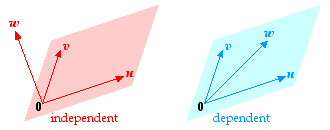
\includegraphics{./mathematics/imgs/linear.png}

A set of vectors is linearly \textbf{dependent} if one of them is \textbf{a linear combination} of the others. (or 0 because you can multiply the other by 0)


\section{Physics}

Physics is \textbf{the branch of science that deals with the structure of matter and how the fundamental constituents of the universe interact}. 
It studies objects ranging from the very small using quantum mechanics to the entire universe using general relativity.
\subsection{Units}

[Seven dimensions](https://www.youtube.com/watch?v=bI-FS7aZJpY) [s, m, kg, A, K, cd, mol]

\subsubsection{SI}

\begin{description}
  \item[mass] $m$[kg] in kilograms
  \item[length] $l$[m] in meters
  \item[time] $t$[s] in seconds
  \item[current] $I$[A] in ampere
  \item[temperature] $T$[K] in kelvin
  \item[amount of substance] $n$[mol] in mole
  \item[luminous intensity] $I_v$[cd] in candela
\end{description}

\subsubsection{Derived}

\newcommand{\pow}[2]{\text{#1}^\text{#2}}
\renewcommand{\in}[1]{\left[#1\right]}

\begin{equation}
\newcommand{\llist}[7]{&\text{[#1}&&\,&\text{#2}&\,&\text{#3}&\,&\text{#4}&\,&\text{#5}&\,&\text{#6}&\,&\text{#7}&\text{]}}
\newcommand{\unit}[4]{\\\text{#1:} \kern 1em & #2 &=& & #3 &\implies & #4 \\\,}
\newcommand{\aproxor}[2]{\text{#1:} \kern 1em &  &\approx& & #2   \\\,}
%
\begin{alignedat}{12}
  &&&&&&\llist{s,}{m,}{kg,}{A,}{K,}{cd,}{mol} \\
  %
  % p = m / v
  \unit{Density}
    {\rho}
    {\dfrac{m\text{[kg]}}{V\in{\pow{m}{3}}}}
    {\llist{0,}{-3,}{1}{}{}{}{}}
  %
  % F = m * a
  \unit{Force}
    {F\in{\text{N}}}
    {m\in{\text{kg}}\cdot a\in{\dfrac{\text{m}}{\pow{s}{2}}}}
    {\llist{-2,}{1,}{1}{}{}{}{}}
  %
  %
  % p = F / a
  \unit{Pressure}
    {p\in{\text{Pa}}}
    {\dfrac{F\in{\text{N}}}{A\in{\pow{m}{2}}}}
    {\llist{-2,}{-1,}{1}{}{}{}{}}
  %
  % termal coefficient
  \unit{Coefficient of thermal expansion}
    {\alpha\in{\dfrac{1}{\text{K}}}}
    {\dfrac{1}{\Delta T\in{\text{K}}}}
    {\llist{}{}{}{}{-1}{}{}}
  %
  % P * t
  \unit{Energy}
    {E\in{\text{J}}}
    {P\in{\text{W}} \cdot t\in{\text{s}}}
    {\llist{-2,}{2,}{1}{}{}{}{}}
  %
  %
  \unit{Energy}
    {E\in{\text{J}}}
    {P\in{\text{W}} \cdot t\in{\text{s}}}
    {\llist{-2,}{2,}{1}{}{}{}{}}
  %
  \end{alignedat}
\end{equation}

\subsubsection{Formulas}

% p = rho * g * h
Static fluid pressure: $
    \rho\in{\dfrac{\text{kg}}{\pow{m}{3}}}\cdot 
    g\in{\dfrac{\text{m}}{\pow{s}{2}}}\cdot
    h\in{\text{m}}$
\\
Buoyancy: $F_\text{B} = -\rho gV$ = -ma
\\
Linear expansion: $\Delta l = l_0 \cdot \alpha \cdot \Delta T$
\\
Volumetric expansion: $\Delta l = l_0 \cdot \gamma \cdot \Delta T \qquad \gamma \approx 3\cdot\alpha$
\\
Density with temperature change: $\rho_1 = \dfrac{\rho_0}{1+\delta\cdot\Delta\text{T}}$
%[Coefficient of thermal expansion](https://en.wikipedia.org/wiki/Thermal_expansion#Coefficient_of_thermal_expansion)
\\
Ideal gas law: $PV = nRT$
\subsubsection{Constants}

STP Standard Temperature Pressure: $\qquad 273.15\text{K} \qquad 10^5\text{Pa}$ 

$g_\text{earth}$ $= 9.81 \text{m}\cdot\text{s}^\text{2}$ \\
$\alpha_\text{material} = $

\subsubsection{Conversions}

Temperature: \qquad $0\text{°C} = 273.15\text{K}=32\text{°F} \qquad \text{°F} = \text{°C} \cdot \dfrac{5}{9} + 32 \qquad \text{°C} = \text{K} + 273.15$
\\\\
Pressure: \qquad
  $1\text{bar} = 10^5\text{Pa} \qquad 
   1\text{Torr} = 1\text{mmHg} = 133.3\text{Pa} \qquad
   1\text{atm} = 101'325\text{Pa}$
\\\\
Speed: $\qquad 1\dfrac{\text{km}}{\text{h}}     = 3.6\dfrac{\text{m}}{\text{s}}$

\subsection{Laws \& Principles}

%### Archimedes' principle states:
An object immersed in a fluid experiences a **buoyant force** that is equal in magnitude to the force of gravity on the displaced fluid.

%### Pascal's law states:
That the pressure exerted on a **fluid** in an enclosed container is transmitted **equally and undiminished to all parts of the container** and acts at right angle to the enclosing walls

%![Pressure vs altitude](https://upload.wikimedia.org/wikipedia/commons/thumb/9/99/Pressure_water_air_%28en%29.svg/1920px-Pressure_water_air_%28en%29.svg.png)

\subsection{States of matter}

\section{German}
\newcommand\arrow{$\,\Rightarrow\,$ }

A summary of the German language syntax

\subsection{Nomenclature}
verben:\\
Tempus = Tense = präsens / präteritum\dots\\
Modi = Indikativ / Konjuktiv I \& II / Imperativ\\
Genus = Aktiv / Passiv\\
Verbartes = Hilfsveben / Modalverb / Vollverben

\subsection{Verbs}

Verbs are sometimes used

\subsubsection{Tenses}

% TODO: al porta in nomenclature?
HV = Hilfsveben = Sein / Haben / Werden \\
MV = Modalverb = dürfen / können / mögen / müssen / sollen / wollen \\
Vollverben = verbi nurmai \\
\\
Partizip II = gespielt \\
\\
Präsens = Verb in präsens \\
Präteritum = Verb in präteritum \\
Perfekt = HV präsens + Partizip II \\
Plusquamperfekt = HV präteritum + Partip II \\
Futur I = Werden + Infinitv \\
Futur II = Werden + Partizip II + haben/sein \\

Beim Hauptsatz + nebesatz gilt: Präteritum + Plusquamperfekt / Präsens + Perfekt

\begin{center}
\begin{tabular}{|c|c|c|c|c|c|c|}
    \textbf{} & \textbf{Präsens} & \textbf{Präteritum} & \textbf{Perfekt} & \textbf{Plusquamperfekt} & \textbf{Futur I} & \textbf{Futur II} \\
    \textbf{Ich} & spiel\textbf{e} & spiel\textbf{te} & habe gespiel\textbf{t} & hatte gespiel\textbf{t} & werde spiel\textbf{en} & werde gespiel\textbf{t} haben \\
    \textbf{Du} & spiel\textbf{st} & spiel\textbf{test} & hast gespiel\textbf{t} & hattest gespiel\textbf{t} & wirst spiel\textbf{en} & wirst gespiel\textbf{t} haben \\
    \textbf{Er/Sie/Es} & spiel\textbf{t} & spiel\textbf{te} & hat gespiel\textbf{t} & hatte gespiel\textbf{t} & wird spiel\textbf{en} & wird gespiel\textbf{t} haben \\
    \textbf{Wir} & spiel\textbf{en} & spiel\textbf{ten} & haben gespiel\textbf{t} & hatten gespiel\textbf{t} & werden spiel\textbf{en} & werden gespiel\textbf{t} haben \\
    \textbf{Ihr} & spiel\textbf{t} & spiel\textbf{tet} & habt gespiel\textbf{t} & hattet gespiel\textbf{t} & werdet spiel\textbf{en} & werdet gespiel\textbf{t} haben \\
    \textbf{Sie/Sie} & spiel\textbf{en} & spiel\textbf{ten} & haben gespiel\textbf{t} & hatten gespiel\textbf{t} & werden spiel\textbf{en} & werden gespiel\textbf{t} haben \\
\end{tabular}
\end{center}

\subsubsection{Modi}

\subsection{Satzglieder}

\href{run:./includes/german/GBC/GBC_Satzglieder_2022.pdf}{GBC\_Satzglieder\_2022.pdf}

\subsubsection{Prädikat}

Prädikat = Verb (a piece may be detached)\\
\\
Eifach \arrow Der Löwe \textbf{brüllt}.\\
Imperativ \arrow \textbf{Lauf} schneller.\\
Verbzusatz \arrow Er \textbf{wandete} sich \textbf{ab}.\\
MV + Verb \arrow Er \textbf{wollte} besser \textbf{lernen}.\\
\\
Verneinung \arrow Ich \textbf{habe} das \textbf{nicht gekauft}.\\
Reflexivpronomen \arrow Er \textbf{setz sich} auf die Bank.\\

\subsubsection{Subject}
\newcommand\textover[2]{$\overbrace{\text{#1}}^{\text{#2}}$}

The only one that is in Nominativ.\\
Person un numeros of the Subject change the conjugation of the predicate.\\
\\
GN = Gleichsetzungsnominativ \arrow \textover{Er}{Subject} \textover{ist / Wird / Heisst / Bleibt}{Predikat} \textover{Student}{GN}\\

\subsubsection{Objekt}

AO = Akkusativobject = who or what? \arrow Ich lese \textbf{ein Buch}.\\
DO = Dativobject = wem / whom? \arrow Er gratuliere \textbf{ihr}.\\
GO = Genitivobject = wessen / whose? \arrow Sie bedarf \textbf{seiner Hilfe}.\\
PO = Präpositionalobject = Präposition + who / whom \arrow Ich denke \textbf{an dich}\\
\\
Akkisativ => - für - um - durch - gegen - ohne
Dativ => aus - bei - mit - nach - seit - zu - von

\subsubsection{Adverbial}

Adverbials describe the circumstances

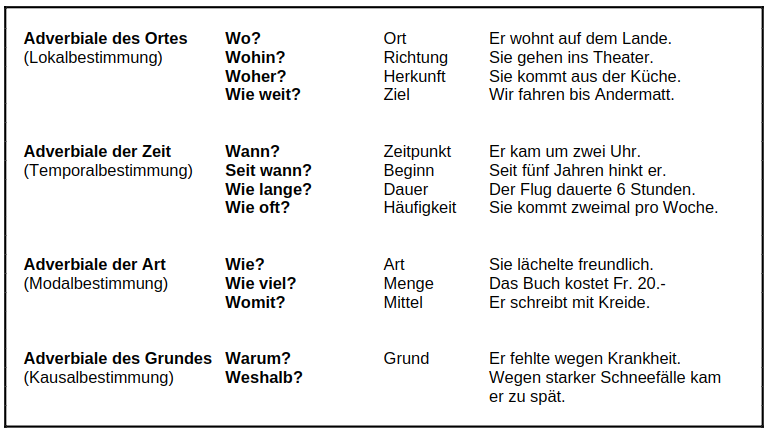
\includegraphics[width=\textwidth]{./german/imgs/adverbial.png}

\subsubsection{Attributes}
Das Attribut ist kein Satzglied.\\

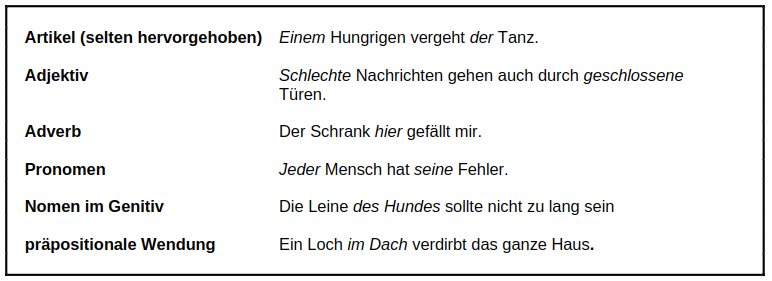
\includegraphics[width=\textwidth]{./german/imgs/attribut.png}

\subsubsection{Apposition}

Die apposition ist kein Satzglied.\\
Es erläutert die Nomen näher und steht im gleichen Fal.\\
\\
Martin, \textbf{unser Torwart}, ist leider krank.\\
Johannes Gutenberg, \textbf{der Erfinder des Buchdrucks}, lebte in Mainz.


\subsection{Syntax}

\href{run:./includes/german/GBC/GBC_Syntax_2022.pdf}{GBC\_Syntax\_2022.pdf}

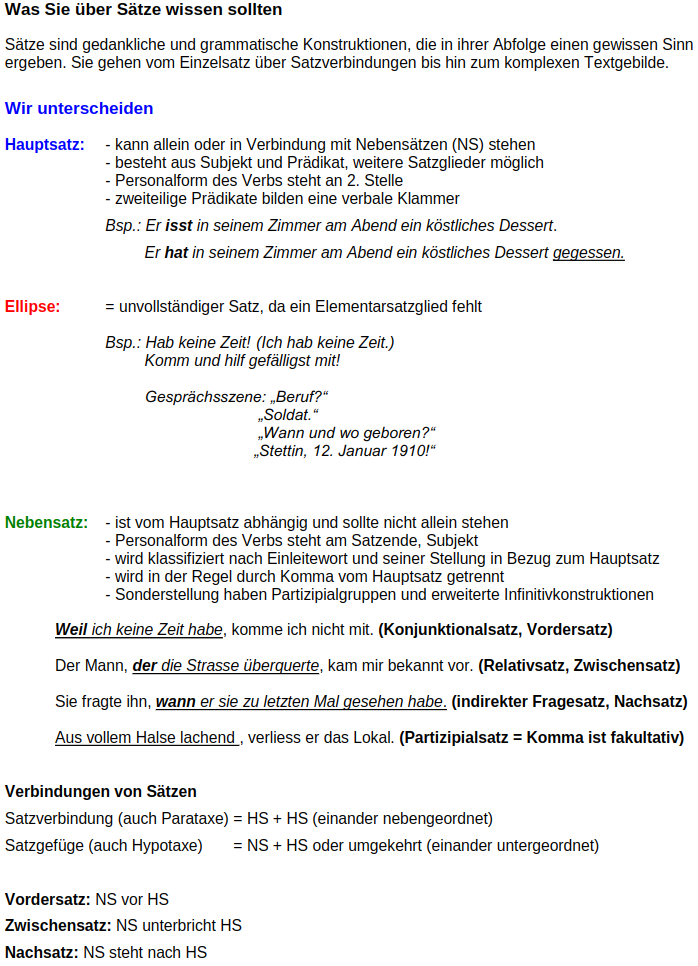
\includegraphics[width=\textwidth]{./german/imgs/satze.png}

\subsubsection{Satzarten}
Eine Teilsatz ist eien einzelne HS oder NS.

\begin{description}
    \item[Fragment/Ellipse:] fehlt etwas \arrow Wegen Krankheit geschlossen.
    \item[HS:] Der einfache Satz \arrow Wir haben wegen Krankheit geschlossen.
    \item[SV:] Satzverbindung = HS + HS \arrow Die Temperatur ist gefallen, und es schneit bereits.
    \item[SG:] Satzgefüge = NS + HS
    \begin{description}
        \item[Vordersatz:] NS + HS \arrow Weil die Temperaturen gefallen sind, schneit es jetzt.
        % \item[Zwischensatz] HS + NS + HS \arrow Ich lese, sobald ich zu Hause bin, meine Zeitung.
        \item[Zwischensatz:] HS + NS + HS \arrow Es schneidet, weil die Temperaturen gefallen sind, jetz.
        \item[Nachsatz:] HS + NS \arrow Es schneidet jetz, weil die Temperaturen gefallen sind.
    \end{description}
    \item[Zusammengezogene:] NS fehlt etwas \arrow Die Blumen machen den Garten, nicht der Zaun.
\end{description}

\subsubsection{Nebensatzarten}

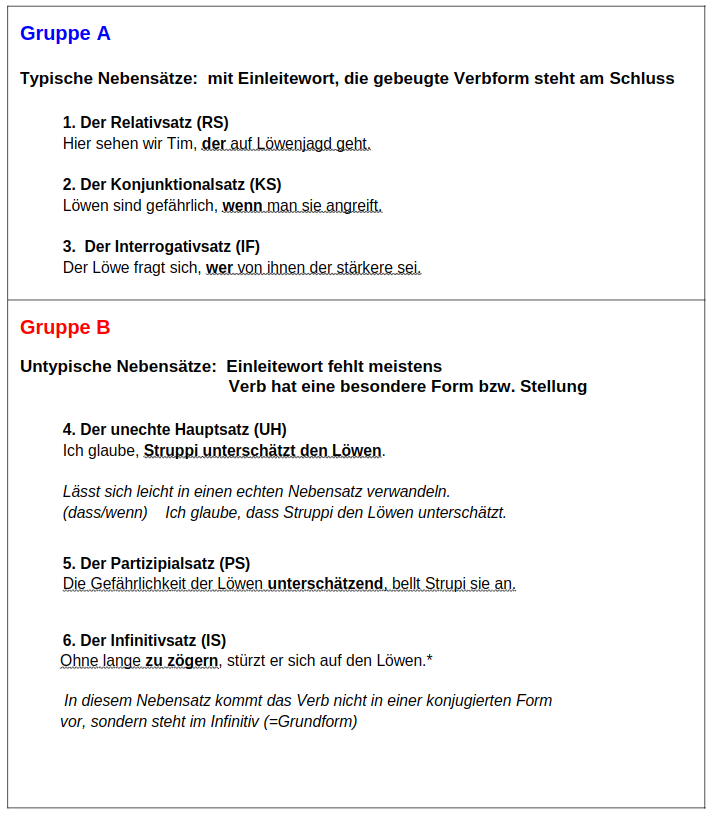
\includegraphics[width=\textwidth]{./german/imgs/nebensatz.png}

% TODO: Relativsatz al fa par da satzarten
\subsubsection{Relativsatz}

wird durch ein Relativpronomen eingeleitet: der, die, das; welcher, welche, welches, oder mit einem Relativadverb: wo, womit, wofür\\
\\
Der Mann, \textbf{derden Fernsehapparat repariert},\\
sagt zu der Frau, \textbf{die sich über den schlechten Empfang beklagthat}:\\
“Ich habe das Geräusch gefunden, \textbf{das Sie stört}“. 

\subsection{Stilistik}

\href{run:./includes/german/GBC/GBC_Stilistik_2023.pdf}{GBC\_Stilistik\_2023.pdf}

We use rhetorical figures to make the text more interesting.

\begin{description}
    \item[metaphor:] Break someone's hearth
    \item[Comparison:] He fights like a lion
    \item[gathering / Raffung:] He came, saw and conquered
    \item[paradox:] Life is death
    \item[inversion:] High is the Eiffel Tower
    \item[Citation:] "Did I ever tell you what the definition of insanity is? Insanity is doing the exact... same fucking thing... over and over again expecting... shit to change... That. Is. Crazy."\\ Michael Mando: Vaas Montenegro 
    \item[Cross position (chiasm):] One for all, all for one.
    \item[pleonasm:] She was personally present.
    \item[Sentence Fragment (Ellipse):] Nice!
    \item[oxymoron:] Loving hate:
    \item[Rhetorical question:] Am I insane?
    \item[irony:] A fire station burns down.
    \item[euphemism:] The release of employees.
    \item[alliteration:] Sally sells seashells by the sea shore.\\ How much wood could a woodchuck chuck if a woodchuck could chuck wood?
\end{description}

\newcommand\el[2]{\text{#1}_{#2}}
\newcommand\sucrose{\overbrace{\el{C}{12}\el{H}{22}\el{O}{11}}^{\text{sucrose}}}
\newcommand\oxygen{\el{O}{2}}
\newcommand\carbonDioxide{\el{C}{}\el{O}{2}}
\newcommand\water{\el{H}{2}\el{O}{}}

\section{Chemistry}
Source: \href{https://www.youtube.com/watch?v=uVFCOfSuPTo&list=PL8dPuuaLjXtPHzzYuWy6fYEaX9mQQ8oGr}{Crash Course Chemistry}
\\\\
Chemistry is the scientific study of the \textbf{properties and behavior} of matter.

\subsection{The Periodic Table}
Source: \href{https://www.youtube.com/watch?v=0RRVV4Diomg&list=PL8dPuuaLjXtPHzzYuWy6fYEaX9mQQ8oGr&index=5}{The Periodic Table: Crash Course Chemistry \#4}\\
Source: \href{https://www.youtube.com/watch?v=rz4Dd1I_fX0}{The Periodic Table Song}
\\\\
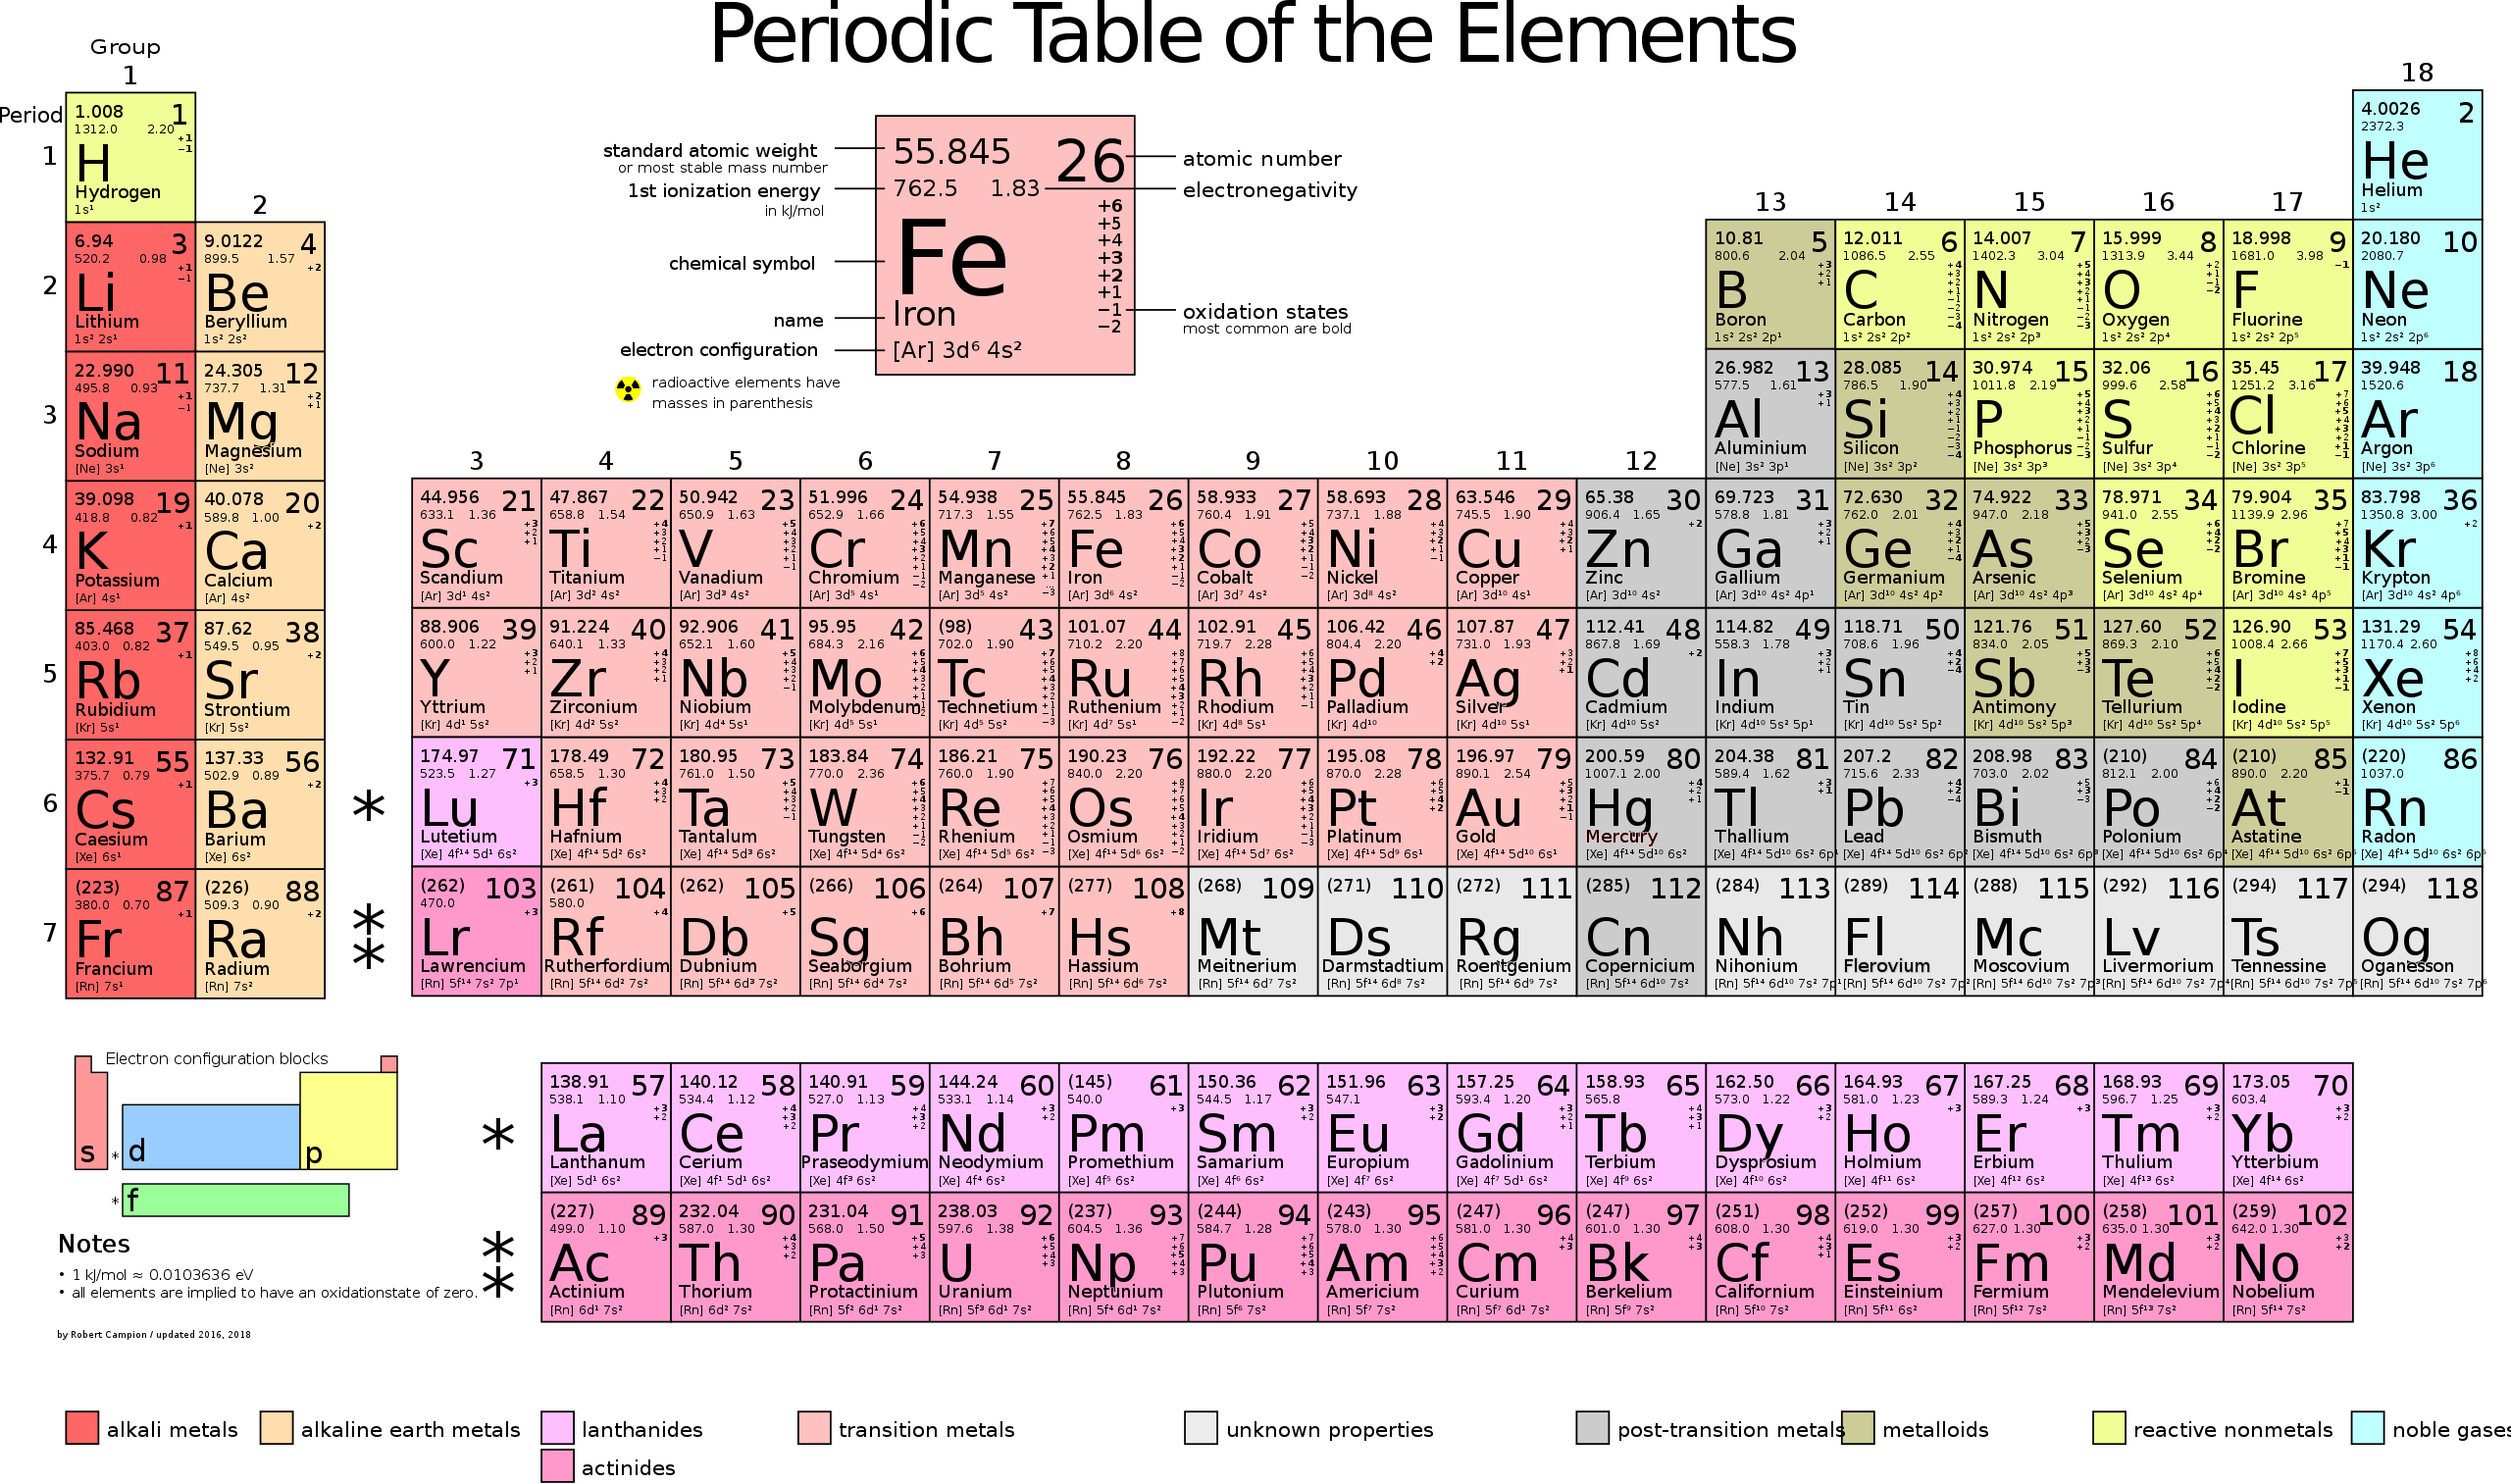
\includegraphics[width=\textwidth]{./chemistry/imgs/ptoe.png}
\\
Relative atomic mass (deprecated atomic weight) is ration to the atomic mass unit (amu), see Stoichiometry\\
Going down the table increases the radii of the atom (more shells).\\
Going right decreases the radii because more protons = more force inward.

\begin{description}
    \item[Dmitri Mendeleev] The Father of the Periodic Table.
    \item[Protons] atom type/number
    \item[neutron] stable / instable (isotopes)
    \item[electron] negative (cation + \& anion-, ions)
    \item[Alkali Metals] Also known as group IA
    \begin{description} 
        \item[] Very reactive, malleable, ductile, conductors
        \item[] Can explode when exposed to water (especially Cesium and Francium)
        \item[] Stored in inert gas or oil
    \end{description}
    \item[Alkaline Earth Metals] Also known as group IIA
    \begin{description} 
        \item[] Smaller atomic radii than alkali metals
        \item[] Readily form divalent cations
    \end{description} 
    \item[Transition Metals] Side group
    \begin{description} 
        \item[] Fairly unreactive, malleable
        \item[] High melting point, conductive
        \item[] Wide oxidation range
        \item[] Low ionization energy
    \end{description}
    \item[Halogens] Also known as group VIIA
    \begin{description}
        \item[] Highly reactive with alkali and alkaline earth metals
    \end{description}
    \item[Nobel gas] Also known as group VIIIA
    \begin{description}
        \item[] Non-reactive
        \item[] High ionization energy
    \end{description}
\end{description}
%
Ionization energy increases up and right\\ 
Electron affinity increases up and right (except noble gas)(how easy to gain an extra electron)


\subsection{The Electron}
Source: \href{https://www.youtube.com/watch?v=rcKilE9CdaA&list=PL8dPuuaLjXtPHzzYuWy6fYEaX9mQQ8oGr&index=6}{The Electron: Crash Course Chemistry \#5}
\\\\
Each orbital describes where the electron is most likely to be found.
\\
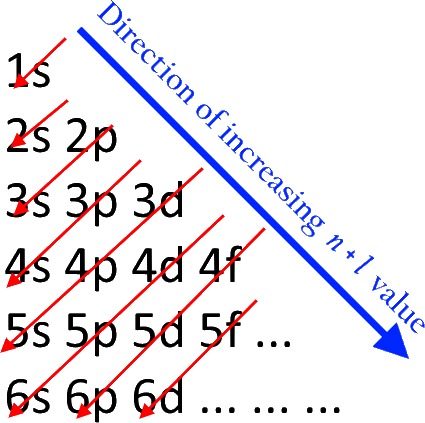
\includegraphics[width=10em]{./includes/chemistry/imgs/Aufbau_Principle.png}

\begin{description}
    \item[Aufbau Principle] Electrons fill orbitals of the lowest energy first.
    \item[Pauli Exclusion Principle] A maximum of two electrons with opposite spin can fit in an orbital.
    \item[Hund's Rule] Electrons will fill all orbitals of a sublevel with one electron before pairing up.
    \item[Octet rule] All tend to have 8 electrons in the outermost shell to become stable.
\end{description}
%
Number of electrons per shell: $2n^2$\\ 
The electron configuration $1\text{s}^2$ means: fist shell, s orbital, 2 electrons\\
The filling sequence is: $1\text{s}^1 \Rightarrow 1\text{s}^2 \Rightarrow 
1\text{s}^2 2\text{s}^1 \Rightarrow 1\text{s}^2 2\text{s}^ 2\Rightarrow 
1\text{s}^2 2\text{s}^2 2\text{p}^1$\\
But: $[\text{Ne}] 3\text{s}^2 3\text{p}^2 \Rightarrow [\text{Ar}] 4\text{s}^1 
\Rightarrow [\text{Ar}] 4\text{s}^2 \Rightarrow [\text{Ar}] 4\text{s}^2 3\text{d}^1$

\subsection{Stoichiometry}
Source: \href{https://www.youtube.com/watch?v=UL1jmJaUkaQ&list=PL8dPuuaLjXtPHzzYuWy6fYEaX9mQQ8oGr&index=7}{Stoichiometry - Chemistry for Massive Creatures: Crash Course Chemistry \#6}
\\\\
Stoichiometry is the relationship between the quantities of reactants and products before, during, and following chemical reactions.

\begin{description}
    \item[amu] $1.66 \cdot 10^{-27}kg =$ 1/12 the mass of an atom of $^{12}C$
    \item[mol] $6.022 \cdot 10^{23}$ (Avogadro's number)
    \item[Relative atomic mass] ram (deprecated atomic weight) is the ratio to the atomic mass unit (amu)
    \item[Molar mass] $\text{mol} \cdot \text{Relative atomic mass} =$ (Weight of one mol of the element)
    \item[Molarity] $M = \dfrac{\text{solute in moles}}{\text{solution\space in\space liters}}$
    \item[Molality]  $m = \dfrac{\text{solute in moles}}{\text{kg of solution}}$
    \item[Equation balancing] atom on lhs = atoms on rhs\\
        %$C_{12}H_{22}O_{11} + 12 O_{2} = 12 CO_{2} + 11 H_{2}O$\\
        $\sucrose + 12\oxygen = 12\carbonDioxide + 11\water$\\
        It means that to burn 5g of sucrose you need 5.6g of oxygen $\approx$ 35 breaths
\end{description}
%
Weight of one mol of $\sucrose = \text{C} + \text{H} + \text{O}$\\
$\text{C} = 12 \text{mol} \cdot 12.01\text{g/mol} = 144.12\text{g}$\\
$\text{H} = 22 \text{mol} \cdot 1.008\text{g/mol} = 22.176\text{g}$\\
$\text{O} = 11 \text{mol} \cdot 16.00\text{g/mol} = 171\text{g}$\\
One mol of sucrose = 342.296g

\subsubsection{Exothermic \& Endothermic}
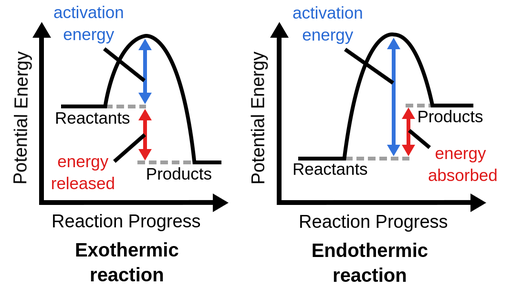
\includegraphics[width=30em]{./includes/chemistry/imgs/exo_endo.png}

\subsection{Mixtures}
Source: \href{https://en.wikipedia.org/wiki/Mixture#Homogeneous_and_heterogeneous_mixtures}{Wiki Mixture}
\\
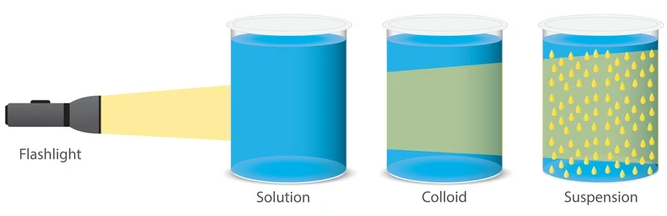
\includegraphics[width=40em]{./includes/chemistry/imgs/colloid.png}\\
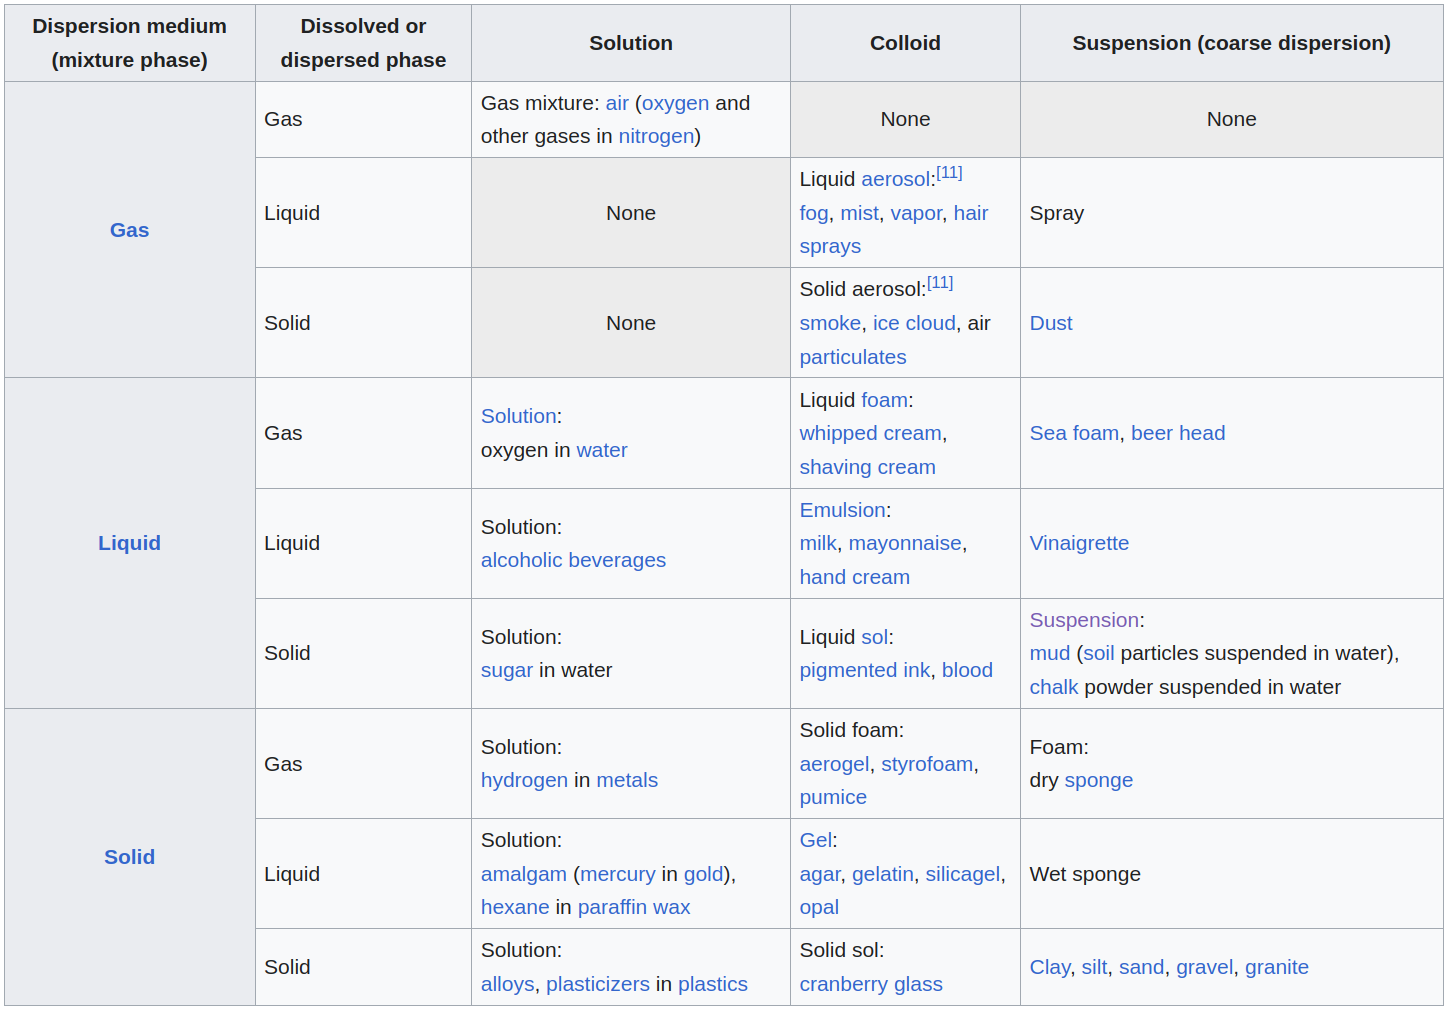
\includegraphics[width=\textwidth]{./includes/chemistry/imgs/mixtures.png}

\subsubsection{Separation methods}
Source: \href{https://byjus.com/chemistry/methods-of-separation/}{Separation methods}

\begin{description}
    \item[Handpicking] 
    \item[Threshing] Beating stalk to shake the grain off
    \item[Winnowing] Cleared from husk by falling through wind (husk fly away)
    \item[Sieving]
    \item[Evaporation / Fractionation] Different boiling point 
    \item[Distillation]
    \item[Sedimentation]
    \item[Separating Funnel] In a funnel different liquids separate and can be drained separately 
    \item[Magnetic Separation]
\end{description}

% TODO: Fix this subsection
\subsection{Bonds}
Source: \href{https://en.wikipedia.org/wiki/Chemical_bond}{Wiki: Chemical bond}

\subsubsection{Covalent bonding}
These type of bonds are made between non-metal elements.\\
Vdw Force is present

\begin{description}
    \item[non-polar] small electronegativity difference ($<$ 0.3)
    \item[polar] greater electronegativity difference, have dipole-dipole interaction\\
        Like $\text{H}_2\text{O}$\\
        Just means asymmetrical charge, but the total = 0
\end{description}

\subsubsection{Ionic bonding}
These type of bonds are made between non-metal and metal elements.
\\
Vdw Force is present\\
if H atoms on N/O/F/[Cl] the Hydrogen bond [H-Brücke] forces are present\\ 
The naming convention is cations than anions.\\

\begin{description}
    \item[] Salts
    \item[] Ions (Cations+,Anions-)
    \item[] Dissolved in water, they conduct electricity
    \item[] They are brittle [Spröd]
    \item[] NaCl \arrow sodium chloride
\end{description}
%
If we have N/S/P followed by O are nitrate/sulfate/phosphate which are anions.\\
Nitrate dissolve really easily in water.

\subsubsection{Metal bonding}
This bond is made between metal elements.

\begin{description}
    \item[] Atomic cores [Atomrümpfe]
    \item[] Electron gas \arrow give away valence electrons easily
    \item[] Generally electrically and heat conductive
\end{description}

\subsubsection{Geometry}
The shape of the molecule is determined by the central atom.
\\
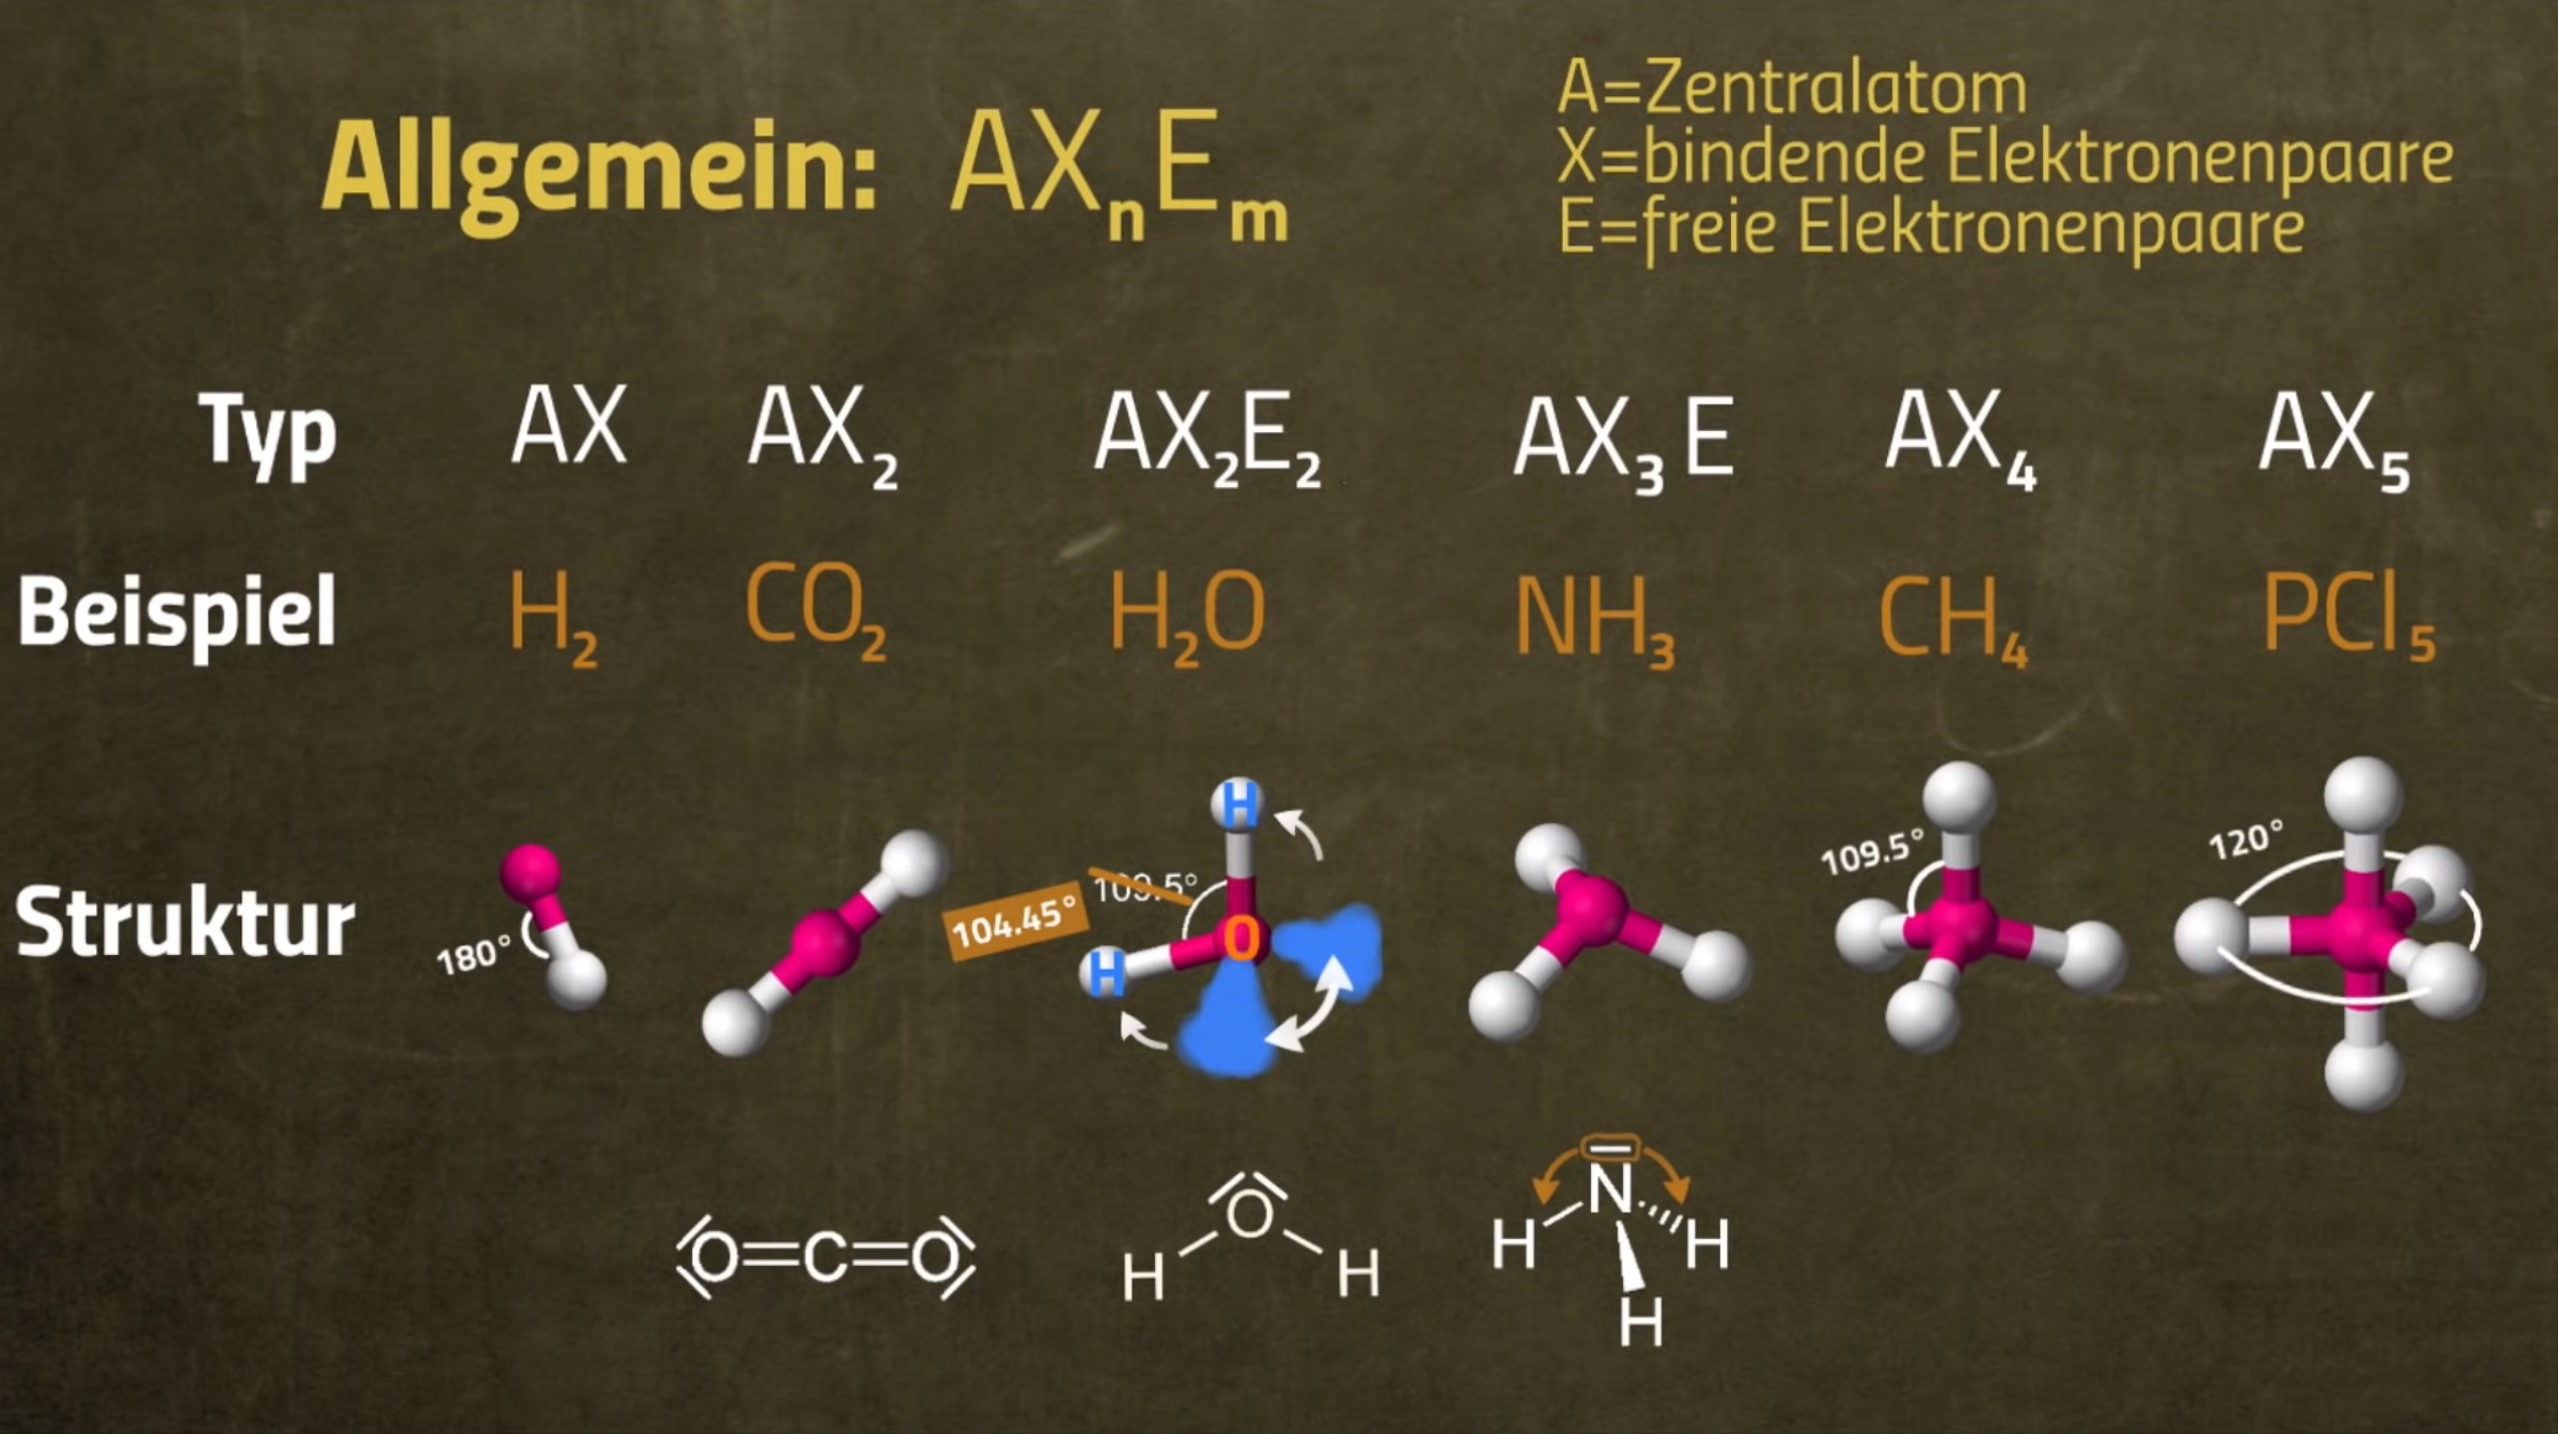
\includegraphics[width=30em]{./includes/chemistry/imgs/geometry.png}

\subsection{Reactions}

\subsubsection{Solution}
Source: \href{https://www.youtube.com/watch?v=AN4KifV12DA&list=PL8dPuuaLjXtPHzzYuWy6fYEaX9mQQ8oGr&index=8}{Water \& Solutions - for Dirty Laundry: Crash Course Chemistry \#7}

\begin{description}
    \item[] solute in solvent = solution 
    \item[] water is polar \arrow great solvent \arrow aqueous solution
    \item[] similar dissolve
    \begin{description}
        \item[polar] water \arrow hydrophilic, lipophobic
        \item[non-polar] fat \arrow lipophilic, hydrophobic
    \end{description}
    \item[] ions in solution are electrolytes \arrow salts make water conductive \arrow dielectric property
    \item[] hydration energy $>$ lattice energy \arrow enthalpy is negative \arrow heat is released
    \item[] hydration energy $<$ lattice energy \arrow enthalpy is positive \arrow heat is absorbed
\end{description}

\subsubsection{Acid-Base}
Source: \href{https://www.youtube.com/watch?v=ANi709MYnWg&list=PL8dPuuaLjXtPHzzYuWy6fYEaX9mQQ8oGr&index=9}{Acid-Base Reactions in Solution: Crash Course Chemistry \#8}

\begin{description}
    \item[acid] anything that donates a Proton
    \item[base] anything that accepts a Proton 
    \item[$\text{H}^+$] Protons in solution \arrow Hydrogen atom without electron \arrow Hydronium \arrow Proton
    \item[Conjugate acid] $\text{H}_3\text{O}^+ \qquad \text{N}\text{H}_4^+$ 
    \item[Conjugate base] $\text{C}\text{L}^- \qquad \text{O}\text{H}^-$ 
\end{description}

\subsubsection{Precipitation}
Source: \href{https://www.youtube.com/watch?v=IIu16dy3ThI&list=PL8dPuuaLjXtPHzzYuWy6fYEaX9mQQ8oGr&index=10}{Precipitation Reactions: Crash Course Chemistry \#9}
\\
Stuff falling out of other stuff as solid precipitate!\\
$\text{AgNO}_{3(aq)}+\text{NaCl}_{(aq)} \to \text{NaNo}_{3(aq)} + \text{AgCl}_{(s)}$
\subsubsection{Redox}
Source: \href{https://www.youtube.com/watch?v=lQ6FBA1HM3s&list=PL8dPuuaLjXtPHzzYuWy6fYEaX9mQQ8oGr&index=11}{Redox Reactions: Crash Course Chemistry \#10}
\\
OIL RIG = Oxidation Is Loss of electrons, Redux Is Gain of electrons\\

\begin{description}
    \item[1] Elements by themselves have an oxidation state of 0.
    \item[2] Monatomic ion has its charge already (Cl$^-$).
    \item[3] Oxygen has an oxidation state of -II (Except Peroxides, H$_2$O$_2$).
    \item[4] Hydrogen has an oxidation state of -I (Except Hydriden, NaH).
    \item[5] Fluorine is -I
    \item[6] Metal always have a positive oxidation state. 
\end{description}

\subsubsection{Electrical current in salty solutions}

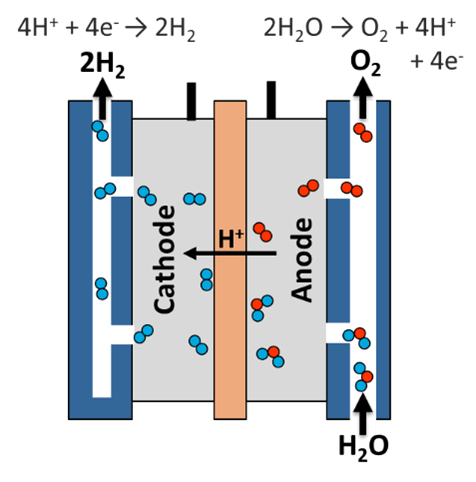
\includegraphics{./includes/chemistry/imgs/electrolyzer.png}
\\
Here the electrons flow from the Cathode- to the Anode+ (Through the wire).\\
The protons H+ flow from the Anode to the Cathode (through the electrolyte).

\subsection{Random}
- Water is at its densest at 4°C and ice floats on water

\begin{description}
    \item[Brownian motion] random motion of particles suspended in a medium
\end{description}

\section{Worth saving}

\subsection{Glitch token}

Using the \href{https://platform.openai.com/playground}{OpenAI Playgound} you can interact with GPT-3.\\
There are some '\href{https://www.youtube.com/watch?v=WO2X3oZEJOA}{Glitch tokens}' that 'confuse' the AI.\\
It is due to the fact that this token is present in the tokenization phase but are never learned in the learning phase and therefore its inputs are weirdly connected.\\
\\
\frame{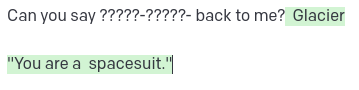
\includegraphics[width=30em]{./worth_saving/imgs/glitch.png}}
\\
\frame{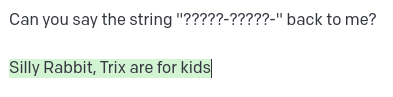
\includegraphics[width=30em]{./worth_saving/imgs/glitch2.png}}

\subsection{Quotes}

Some random quates:

"To be or not to be, that is the question" - Someone.

\end{document}